\section{子研究二:个性化广告效果模型构建} 
在研究一和研究二中,个性化广告的效果评估主要依赖实验数据。尽管 AI 生成技术显著降低了实验材料的制作成本,使大规模生成个性化广告成为可能,但广告效果的验证仍需大量被试,并要求他们填写人格问卷,以匹配个性化广告的目标群体。然而,这种基于实验的方法不仅在时间和资源上存在限制,难以实现快速评估,还需要依赖受试者的参与,因而在实际应用中具有一定局限性。因此,构建预测模型能够提供一种更高效的评估手段,使研究者或广告实践者在广告发布前预测其对不同人格特质群体的吸引力。这不仅有助于降低实验成本,还能在广告投放前优化个性化策略,从而提高广告匹配度和转化率。此外,在前述研究中,我们已收集了大量基于 AI 生成的广告文本,并获得了带有个性化特质信息的被试评分数据,使得构建个性化广告说服效果模型成为可能。尽管实验中的广告是围绕某一特定人格特质(如高外倾性、高开放性等)进行定制的,但广告文本可能包含多层次的语言元素,使其不仅对目标特质群体有效,也可能吸引其他人格特质的个体。例如,一个为高开放性个体设计的广告可能突出探索性与创造力,但其中的情感化或社交化表达同样可能对高宜人性或高外倾性的个体产生吸引力。因此,在模型构建过程中,我们不仅考察广告在目标特质群体中的说服效果,还计算该广告对其他人格特质个体的吸引程度。这一方法突破了传统个性化广告评估仅关注目标群体的局限,使得模型能够更全面地预测个性化广告在不同人格特质群体中的适用范围,为广告优化和投放策略提供更具适应性的参考。综上所述,子研究二基于前述实验的实验材料和数据,结合LIWC语言特征,构建个性化广告效果的预测模型。

\subsection{方法}

\subsubsection{建模数据}

\textbf{(1)数据来源}

本研究的模型构建基于研究一和研究二的实验数据,涵盖 AI 生成与人类专家创作的个性化广告文本及其参与者评分。所有实验均采用大五人格测量工具(BFI-10 或 BFI-44)评估参与者的人格特质,并要求他们对不同个性化广告文本进行评分。为确保模型能够准确评估广告对不同人格特质群体的吸引力,我们优先选取完成完整人格测量的实验数据,以提高个性化说服效果计算的精度。具体而言,模型训练数据整合了多个实验的数据集(详见表 \ref{tab:model_data}),每名参与者在实验中评价 5 条广告,而每条广告的最终评价人数因实验条件不同而有所变化。经过筛选,最终用于模型训练的广告样本共计112条。

\begin{table}[htbp]
    \centering
    \caption{\label{tab:model_data} 建模数据来源}
    {\tablesongti % 整个表格环境应用宋体六号字体
    \renewcommand{\arraystretch}{1.5} % 调整行距
    \begin{tabular}{p{2cm} p{2cm} c c c} % 控制列宽
        \toprule
        \textbf{实验} & \textbf{人格测量量表} & \textbf{参与者人数} & \textbf{每名受试者评价文本数} & \textbf{单条广告评价人数} \\
        \midrule
        研究一-实验1 & BFI-10 & 192 & 5 & 65 \\
        研究二-实验1 & BFI-10 & 322 & 5 & 32--59 \\ % 使用 -- 代替 –
        研究二-实验2 & BFI-44 & 368 & 5 & 13--68 \\ % 使用 -- 代替 –
        \bottomrule
    \end{tabular}
    }
\end{table}




\textbf{(2)计算方法}
\label{calculationMethods}

为构建模型,我们对个性化广告的说服效果进行了量化处理。计算过程分为\textbf{个体层面}和\textbf{广告层面}。

在\textbf{个体层面},我们首先对每名受试者在实验中的广告评分进行标准化,以消除个体评分偏差。随后,将个体的人格得分也进行标准化,并计算个体在所有广告上的评分与其在人格上的偏离程度,以衡量特定人格水平个体对广告的偏好倾向。具体计算如下,其中,\( S_{\text{ad},i} \) 代表个体 \( i \) 在某条广告上的评分,\( \mu_{S,i} \) 和 \( \sigma_{S,i} \) 分别为该个体在所有广告上的评分均值和标准差。类似地,\( P_{i} \) 代表个体 \( i \) 在该人格特质上的得分,\( \mu_{P} \) 和 \( \sigma_{P} \) 分别为该特质在所有被试中的均值和标准差。

\begin{equation}
    Z_{\text{ad},i} = \frac{S_{\text{ad},i} - \mu_{S,i}}{\sigma_{S,i}}, \quad
    Z_{\text{trait},i} = \frac{P_{i} - \mu_{P}}{\sigma_{P}}
    \label{eq:standardization}
\end{equation}

然后,在\textbf{广告层面},计算个体对广告的个性化说服效应。我们将所有被试对某条广告的个性化说服效应 \( P_{\text{ad},i} \) 进行累加,得到该广告针对特定人格特质的个性化说服指数,如公式\eqref{eq:persuasion_effect} 所示。其中,\( P_{\text{ad}} \) 的正值表示高水平特质个体更偏好该广告,低水平特质个体更不偏好(即高水平个性化说服效果较强);而负值则表示低水平特质个体更偏好该广告,高水平特质个体更不偏好(即低水平个性化说服效果较强)。

\begin{equation}
    P_{\text{ad},i} = Z_{\text{ad},i} \times Z_{\text{trait},i}
    \label{eq:persuasion_effect}
\end{equation}

\begin{equation}
    P_{\text{ad}} = \sum_{i=1}^{N} P_{\text{ad},i}
    \label{eq:persuasion_index}
\end{equation}


\subsubsection{模型选择}
在本研究中,我们选用了随机森林(Random Forest)作为个性化广告说服效果的预测模型。这一选择主要基于其在处理高维数据、特征选择、非线性建模以及对小样本数据的适应性等方面的优势,使其特别适用于文本特征驱动的预测任务。本研究的自变量来源于广告文本的语言特征,因变量则为该广告在不同人格群体中的个性化说服效果。文本特征采用LIWC(Linguistic Inquiry and Word Count)分析得到,涵盖多个维度,如情感(情绪正负性)、认知(推理、因果分析)、社交(人称代词、社交相关词汇)以及驱动(成就动机、亲和动机等)。由于广告文本包含多个层面的语言元素,个性化广告的说服效果可能受到不同语言特征的复杂影响。因此,我们需要一种既能处理高维数据、又能捕捉非线性关系的建模方法,以提高个性化广告预测的准确性。

随机森林模型在这一任务中具有显著优势。首先,它适用于高维特征数据。在文本分析任务中,自变量往往由多个语言特征构成,且不同特征可能存在较强的相关性。相比传统回归模型,随机森林能够在众多特征中自动选择最具预测价值的变量,而不会受到多重共线性问题的困扰。同时,其集成学习机制通过多个决策树的组合,减少了单一模型可能出现的过拟合问题,从而提升泛化能力。

其次,随机森林具备强大的特征选择能力。在个性化广告预测任务中,我们希望不仅能够预测广告的说服效果,还能识别哪些文本特征最具影响力。随机森林能够通过计算特征重要性,如基尼指数(Gini Importance)或置换重要性(Permutation Importance),评估每个文本特征对说服力的贡献。这一特性使得我们能够深入分析不同语言特征在个性化广告中的作用,并据此优化广告文案的个性化策略。

此外,个性化广告的说服效果可能受到多种复杂因素的共同影响。例如,词汇的多样性可能在一定程度上提升广告吸引力,但过度复杂的表达可能降低可读性,从而影响说服效果;具有情感共鸣的语言可能对某些人格特质的个体有效,但对其他群体则可能适得其反;认知类词汇(如逻辑推理、因果分析)可能增强信息可信度,但对低开放性个体来说可能较难理解。相较于线性回归或普通决策树,随机森林能够灵活捕捉这些非线性模式,使得预测模型更贴合文本特征与个性化广告效果之间的真实关系。

另一个关键优势是随机森林对异常值和噪声的鲁棒性。由于文本数据可能包含噪声(如广告文案中的冗余词汇)、极端值(如某些特征的异常高频)或缺失值,随机森林的集成学习方式能有效降低单一异常值对整体预测结果的影响。多个决策树的投票机制确保了模型的稳定性,使其在数据质量不完美的情况下仍能保持较好的预测性能。

最后,随机森林在小样本和不平衡数据下仍能稳定表现。个性化广告的实验数据相较于典型的自然语言处理(NLP)任务而言,规模相对较小,且不同人格特质的受试者分布可能存在不均衡。随机森林的随机采样(Bootstrap Sampling)机制使其能够更好地利用有限数据,并通过集成多个弱学习器提升模型的泛化能力。

\subsubsection{模型训练}
在本研究中,我们采用随机森林分类器(Random Forest Classifier)对个性化广告的说服效果进行建模与训练。模型训练的主要目标是基于广告文本的语言特征,预测该广告在特定人格特质群体中的说服力。具体而言,我们针对大五人格的每个维度分别训练一个分类模型,以评估广告文本在不同人格群体中的个性化效果。在模型训练过程中,我们首先对数据进行划分。对于每个目标人格特质(如开放性、尽责性等),自变量X由 LIWC 语言特征组成,因变量y代表该广告在该人格特质上的个性化说服效果(计算方法详见\ref{calculationMethods})。由于个性化说服得分是一个连续变量,为构建分类模型,我们将其转换为二分类标签:

\begin{equation}
y =
\begin{cases}
1, & P_{\text{ad}} \geq 0 \quad \text{(广告更受高水平特质个体偏好)} \\
0, & P_{\text{ad}} < 0 \quad \text{(广告更受低水平特质个体偏好)}
\end{cases}
\end{equation}

这样,我们的分类模型即可预测某则广告是否更符合高水平特质个体的偏好模式。为确保模型的稳健性,我们将数据集按照7:3的比例划分为训练集(70\%)和测试集(30\%),并采用分层抽样,使得训练集和测试集中各人格特质水平的分布保持一致,以减少类别不均衡对模型的影响。

在训练过程中,我们采用两阶段建模策略,即先训练基础随机森林模型,再利用该模型进行特征选择,以筛选出最具预测价值的语言特征。首先,我们使用100 棵决策树(n\_estimators=100)训练一个初始随机森林分类器,并利用其特征重要性来进行变量筛选。具体而言,我们基于平均特征重要性设定筛选阈值,仅保留重要性高于均值的特征,从而减少冗余信息,提高模型的泛化能力。随后,我们使用筛选后的特征重新训练最终的随机森林分类器,以进一步优化预测性能。训练完成后,我们在测试集上评估模型性能,并计算准确率以衡量模型的预测能力。

\subsection{结果}

\textbf{(1)模型预测结果}

图 \ref{fig:prediction_accuracy} 展示了基于随机森林模型对不同人格特质个性化广告的预测准确率。纵轴表示预测准确率,横轴为五种人格特质(宜人性、外倾性、开放性、尽责性、神经质)。从结果来看,尽责性广告的预测准确率最高(0.76),其次为神经质(0.66)、宜人性(0.65)、外倾性(0.62),而开放性广告的预测准确率最低(0.59)。其中,图中的虚线表示随机水平(即 0.50),若预测准确率高于该水平,说明模型的预测优于随机猜测。整体而言,模型在不同人格特质上均表现出一定的预测能力,尤其是在尽责性广告上的预测效果最佳。这可能与尽责性个性化广告的语言特征更加稳定、可预测性更高有关,而开放性广告的预测效果相对较低,可能是由于其语言风格更加多样化,导致模型难以捕捉固定模式。

\begin{figure}[H]
    \centering
    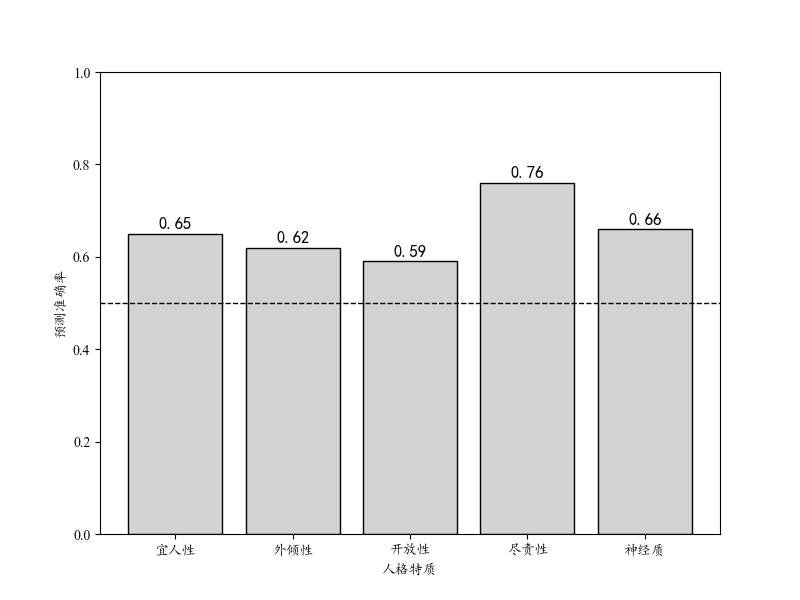
\includegraphics[width=1\linewidth]{Image/Study3-predictionAccuray.png}
    \caption{\label{fig:prediction_accuracy}模型预测准确率}
\end{figure}

为进一步解析个性化广告预测模型中语言特征的作用,本研究引入 SHAP(SHapley Additive exPlanations) 方法对特征贡献进行分析。SHAP 是一种基于 Shapley 值的模型解释方法,被广泛用于评估机器学习模型中各特征对预测结果的贡献。其核心思想是计算每个特征在不同预测情境下的边际贡献,从而提供一致且可解释的特征重要性衡量标准。相比于传统的特征重要性计算方法(如随机森林中的 Gini 重要性或基于置换的重要性分析),SHAP 具有更强的理论可解释性,能够有效捕捉特征间的交互效应,使研究者能够更全面地理解模型的决策过程。

\textbf{(2)特征贡献度}

在本研究中,我们针对五种人格特质(宜人性、外倾性、开放性、尽责性、神经质)分别计算 SHAP 值,以解析不同语言特征在个性化广告预测任务中的贡献。SHAP 值的正负表示该特征对模型预测结果的影响方向:正 SHAP 值表示该特征增加了高水平特质个体偏好的预测概率,而负 SHAP 值则表示该特征更倾向于预测低水平特质个体的偏好模式。此外,SHAP 值的绝对大小反映了该特征的重要性,即数值越大,说明该特征对模型预测的影响越显著。图 \ref{fig:featureHeatmap} 展示了 SHAP 计算得到的特征重要性热力图,横轴表示人格特质类别,纵轴为 LIWC 语言特征,颜色深浅表示该特征在相应人格特质预测任务中的贡献大小。

从 SHAP 计算结果来看,不同人格特质的个性化广告在语言特征上表现出一定的模式。例如,在 \textbf{尽责性} 个性化广告的预测模型中,\textit{drives}(动机相关)、\textit{work}(工作相关)和\textit{quant}(数量表达)等特征的重要性最高,这与尽责性个体强调目标导向、任务执行和条理性的特点一致。同时,\textit{negemo}(负面情绪)特征在尽责性广告预测中也表现出较高 SHAP 贡献,这可能是由于尽责性个体在广告内容中更关注潜在风险或任务挑战,从而影响其对广告的接受度。

在 \textbf{外倾性} 个性化广告的预测模型中,\textit{social}(社交相关)、\textit{posemo}(正面情绪)和\textit{reward}(奖励)等特征的重要性较高,表明外倾性个体更倾向于被强调社交互动、正向体验和激励机制的广告所吸引。此外,\textit{you}(第二人称代词)的贡献也较大,可能表明外倾性个体更偏好直接互动式的广告表达。

\textbf{宜人性} 个性化广告的预测模型则显示,\textit{compare}(比较)、\textit{motion}(运动相关)和\textit{feel}(情感相关)等特征的重要性较高。这表明宜人性个体在广告中更关注人与人之间的关系、情感共鸣以及相对评价,而\textit{pronoun}(代词)的贡献也说明宜人性广告可能更倾向于使用第一人称或第三人称代词,以增强广告的亲和力和人际互动。

\textbf{神经质} 个性化广告的预测模型中,\textit{negemo}(负面情绪)、\textit{tentat}(不确定性)和\textit{risk}(风险)等特征的重要性最高。这表明神经质个体更倾向于受到涉及焦虑、不安和不确定性表达的广告影响,同时也可能偏好那些能够提供安全感和情绪安抚的信息。此外,\textit{social}(社交相关)特征在神经质个体的广告预测中也具有较高贡献,这可能是由于该群体更容易受到社交焦虑或社交互动内容的影响。

相比之下,\textbf{开放性} 个性化广告的预测模型中,各特征的 SHAP 贡献较为分散,缺乏单一主导特征。这可能与开放性人格本身的语言风格高度多样化有关。例如,\textit{informal}(非正式表达)、\textit{cause}(因果逻辑)、\textit{cogproc}(认知过程)和\textit{compare}(比较)等特征在开放性广告预测中均有所贡献,但整体重要性不如其他人格特质广告任务中的显著。这一结果可能表明,开放性广告的个性化表达方式较为宽泛,使得模型难以精准捕捉统一的语言模式。

综合来看,SHAP 分析进一步支持了 LIWC 语言特征在个性化广告预测中的作用,并揭示了不同人格特质在语言表达上的独特性。尽责性、外倾性和宜人性广告的语言特征较为稳定,使得模型能够较准确地预测个性化广告效果,而开放性广告由于语言多样性较高,可能导致预测性能的下降。这一发现不仅为 AI 生成个性化广告的优化提供了数据支持,也为未来在个性化广告设计中更精细地调整语言策略提供了理论依据。

\begin{figure}[H]
    \centering
    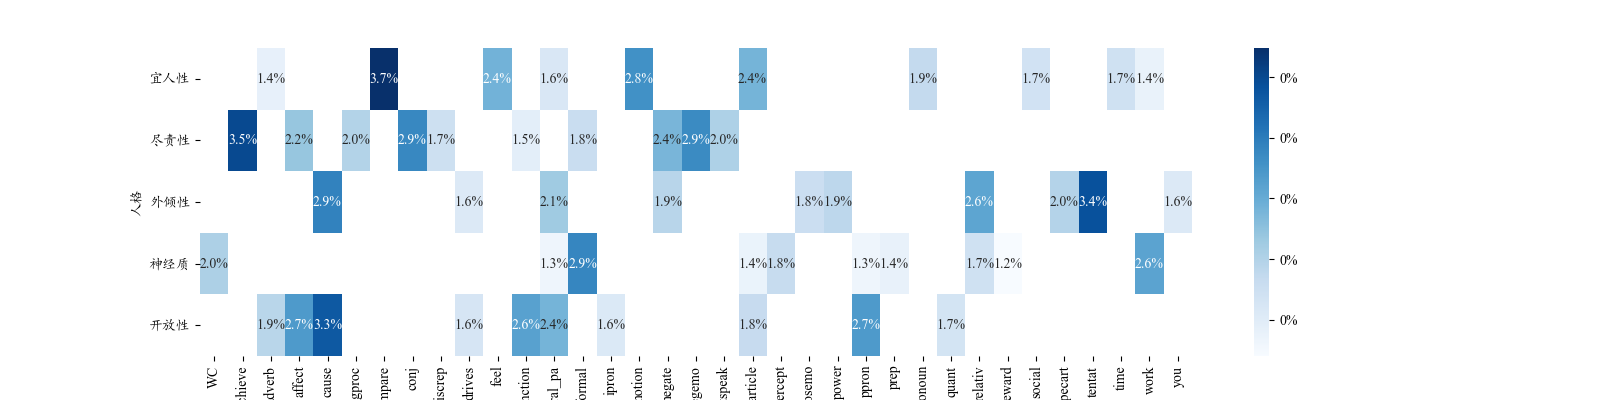
\includegraphics[width=1.2\linewidth]{Image/Study3-heatmap.png}
    \caption{\label{fig:featureHeatmap}特征SHAP值热力图}
\end{figure}

\textbf{(3)高水平vs低水平偏好特征差异}

在本研究中,我们基于参与者的实际广告评分计算了个性化说服效应(计算方法详见 \ref{calculationMethods}),衡量不同人格特质水平的个体对广告内容的偏好模式。相较于子研究一仅关注高水平特质广告文本的语言特征(§ \ref{study3-substudy1}),本研究中进一步分析高低水平人格特质个体在广告语言特征上的偏好差异。通过独立样本t检验比较高水平与低水平个体在LIWC 语言特征偏好上的显著性差异,并计算 Cohen’s d以评估效应量。这一分析不仅揭示了高低水平个体在广告接受度上的语言特征偏好,还为优化个性化广告的匹配策略提供了新的视角。

高宜人性个体更偏好包含 \textbf{比较(compare)} 词汇的广告 \((t = 3.13, p = 0.002, d = 0.59)\),并且在\textbf{代词(pronoun)} 使用上显著更高 \((t = 2.65, p = 0.009, d = 0.50)\)。这表明,高宜人性个体更倾向于接受\textbf{强调个体差异、相对优势} 的广告,例如:“你的时间宝贵,所以我们的手机不容许任何延误。一键快速响应,确保每一秒都计算得刚刚好。” 此外,高宜人性个体对\textbf{未来导向(focusfuture)} 的内容表现出更高的接受度 \((t = 1.97, p = 0.052, d = 0.37)\),说明他们更偏好\textbf{强调长期利益和积极愿景} 的广告表达。低宜人性个体更偏好\textbf{否定(negate)} \((t = -2.04, p = 0.044, d = -0.39)\) 和\textbf{愤怒(anger)} \((t = -2.01, p = 0.049, d = -0.39)\),表明他们对\textbf{直接、批判性更强的广告} 反应更积极,如:“你的朋友已为此狂热,这不仅是手机,更是社交的新纪元。展现个性,享受交流,无限精彩尽在掌中。” 此外,低宜人性个体对\textbf{生物相关词汇(bio,如“健康”“身体”)} 更敏感 \((t = -2.15, p = 0.035, d = -0.42)\),这可能意味着他们更容易被\textbf{与身体机能、健康维护相关的广告} 吸引,如:“智能调节屏幕色温,缓解视疲劳,让工作休闲更加舒适。”

高开放性个体在\textbf{代词(ppron)} \((t = 2.91, p = 0.004, d = 0.55)\) 和\textbf{功能词(function words)} \((t = 2.26, p = 0.026, d = 0.43)\) 的使用上显著更高,表明他们更倾向于接受\textbf{强调个体体验、社交互动,或富有思辨性的广告表达},例如:“使用这款手机,你将体验到最全新的技术、最前卫的设计;在这里,你将以从未想象过的方式探索手机的世界。” 此外,高开放性个体更偏好\textbf{强调集体归属感} 的语言,他们更常被包含 \textbf{“我们”(we)} 的广告所吸引 \((t = 2.06, p = 0.042, d = 0.39)\),如:“共同追求进步,创造美好的明天。手机作为你的工具,与你一同实现梦想。” 低开放性个体更偏好\textbf{数字(number)} \((t = -1.93, p = 0.058, d = -0.36)\),说明他们更倾向于\textbf{基于数据、事实支撑的广告},例如:“99\% 的用户推荐,实验数据显示出色性能。”

高尽责性个体更偏好\textbf{功能词(function)} \((t = 2.70, p = 0.008, d = 0.52)\) 和\textbf{未来导向(focusfuture)} \((t = 1.83, p = 0.070, d = 0.34)\),表明他们更容易接受\textbf{逻辑清晰、目标导向的广告},例如:“精准定位,发现生活中的美好细节。捕捉时刻,记录珍贵瞬间。” 低尽责性个体更偏好\textbf{否定(negate)} \((t = -2.54, p = 0.013, d = -0.50)\) 和\textbf{负面情绪词汇(negemo)} \((t = -2.46, p = 0.016, d = -0.47)\),说明他们更容易被\textbf{强调挑战、失败或压力} 的广告吸引,如:“如果你不立即采取行动,你可能会错失机会。”

高外向性个体更偏好\textbf{相对性词汇(relativ,如“更快”“更高”)} \((t = 2.58, p = 0.011, d = 0.49)\) 和\textbf{不确定性表达(tentat,如“可能”)} \((t = 2.45, p = 0.016, d = 0.46)\),他们更容易接受\textbf{强调探索性、互动感的广告},如:“翻阅朋友的动态,把温馨的友情牢牢捕捉。” 低外向性个体 更偏好\textbf{权力(power)} 相关词汇 \((t = -2.08, p = 0.041, d = -0.40)\),表明他们更倾向于\textbf{强调掌控感、决策权威性的广告},如:“你的时间宝贵,所以我们的手机不容许任何延误。”

高神经质个体偏好\textbf{网络用语(netspeak)} \((t = 2.00, p = 0.050, d = 0.40)\),表明他们更容易接受\textbf{非正式、口语化的广告风格},如:“在欢笑中,她是你探索世界的桥梁;在泪水中,她是你疗愈伤痕的港湾。” 低神经质个体更偏好\textbf{未来导向(focusfuture)} \((t = -3.03, p = 0.003, d = -0.57)\),这表明他们更倾向于\textbf{强调长期规划、稳定性的广告},如:“开启智慧生活,助你成为更好的自己。”
